\documentclass[12pt]{article}
\setlength{\oddsidemargin}{0in}
\setlength{\evensidemargin}{0in}
\setlength{\textwidth}{6.5in}
\setlength{\parindent}{0in}
\setlength{\parskip}{\baselineskip}

\usepackage{amsmath,amsfonts,amssymb,bm,graphics,pgfplots,framed,dsfont}
\usepackage[scale=0.75,top=1cm,bottom=3cm]{geometry}

\begin{document}

\textbf{Minh Anh Nguyen }\\
\textbf{Calculus 1 Assignment-10}\\
\textbf{Section: 04}\\
\textbf{TA's name: Arthur Huey}

\hrulefill

\begin{enumerate}
\setcounter{enumi}{6}
    \item A table of values of an increasing function $f$ is shown. Use the table to find the lower and upper bound estimates of $\int_{10}^{30} f(x)dx$
    \begin{center}
        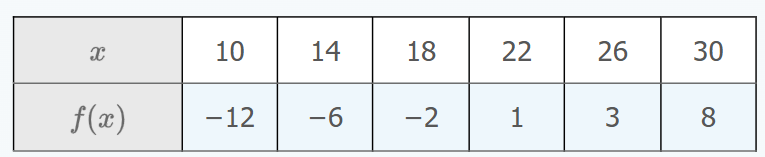
\includegraphics[scale=0.5]{img/img-0.png}
    \end{center}
    \[Lower = 4\times(-12 + -6 + -2 + 1 + 3) = -64\]
    \[Upper = 4\times(-6 + -2 + 1 + 3 + 8) = 16\]
\setcounter{enumi}{10}
    \item Use the Midpoint Rule with the given value of $n$ to approximate the integral. Round the answer to four decimal places.
    \[\int_{0}^{8} \sin \sqrt{x} \text{ } dx, n = 4\]
    \[\Delta x = \frac{8-0}{4} = 2\]
    \[\int_{0}^{8} \sin \sqrt{x} \approx 2 \times (f(\frac{2+0}{2}) + f(\frac{4+2}{2}) + f(\frac{6+4}{2}) + f(\frac{8+6}{2})) \approx 6.1820\]
\setcounter{enumi}{18}
    \item Express the limit as a definite integral on the given interval.
    \[\lim_{n \to \infty} \Sigma_{i=1}^{n} \frac{\sin x_i}{1 + x_i}\Delta x, [0,\pi]\]
    \[\lim_{n \to \infty} \Sigma_{i=1}^{n} \frac{\sin x_i}{1 + x_i}\Delta x = \int_{0}^{\pi} \frac{sin x}{1 + x} dx\]
\setcounter{enumi}{22} 
    \item Show that the definite integral is equal to $\lim_{n \to \infty} R_n$ and then evaluate the limit.
    \[\int_{0}^{4}(x-x^2)dx, R_n = \frac{4}{n} \Sigma_{i = 1}^{n}[\frac{4i}{n} - \frac{16i^2}{n}]\]
    \[\Delta x = \frac{4-0}{n} = \frac{4}{n}\]
    \[x_i = \frac{4i}{n}\]
    According to Riemann Sum:
    \[\int_{0}^{4}(x-x^2)dx = R_n = \frac{4}{n} \Sigma_{i = 1}^{n}[\frac{4i}{n} - \frac{16i^2}{n}]\]
    \[R_n = \frac{4}{n} \Sigma_{i = 1}^{n}[\frac{4i}{n} - \frac{16i^2}{n}] = \frac{4}{n} \Sigma_{i = 1}^{n}\frac{4i}{n} - \frac{4}{n} \Sigma_{i = 1}^{n} \frac{16i^2}{n}\]
    \[\frac{4}{n} \Sigma_{i = 1}^{n}\frac{4i}{n} - \frac{4}{n} \Sigma_{i = 1}^{n} \frac{16i^2}{n}\]
\end{enumerate}
\end{document}